\documentclass[journal]{IEEEtran}

% *** CITATION PACKAGES ***
%
%\usepackage{cite}
\usepackage{capt-of}%%To get the caption
\usepackage{gensymb}
\usepackage{graphicx} %package to manage images
\graphicspath{ {./images/} }
\usepackage{wrapfig}

\usepackage{amsmath}


\usepackage[style=ieee]{biblatex}
\DeclareLanguageMapping{english}{english-apa}
\addbibresource{references.bib}
\usepackage[justification=centering]{caption}

\usepackage{setspace}

\usepackage{hhline}


\usepackage{changepage} 

\usepackage{booktabs}
\usepackage{xcolor}

\usepackage{makecell}

\renewcommand\theadfont{}

%\raggedbottom

% *** GRAPHICS RELATED PACKAGES ***
%
\ifCLASSINFOpdf
  % \usepackage[pdftex]{graphicx}
  % declare the path(s) where your graphic files are
  % \graphicspath{{../pdf/}{../jpeg/}}
  % and their extensions so you won't have to specify these with
  % every instance of \includegraphics
  % \DeclareGraphicsExtensions{.pdf,.jpeg,.png}
\else
  % or other class option (dvipsone, dvipdf, if not using dvips). graphicx
  % will default to the driver specified in the system graphics.cfg if no
  % driver is specified.
  % \usepackage[dvips]{graphicx}
  % declare the path(s) where your graphic files are
  % \graphicspath{{../eps/}}
  % and their extensions so you won't have to specify these with
  % every instance of \includegraphics
  % \DeclareGraphicsExtensions{.eps}
\fi
% graphicx was written by David Carlisle and Sebastian Rahtz. It is
% required if you want graphics, photos, etc. graphicx.sty is already
% installed on most LaTeX systems. The latest version and documentation
% can be obtained at: 
% http://www.ctan.org/pkg/graphicx
% Another good source of documentation is "Using Imported Graphics in
% LaTeX2e" by Keith Reckdahl which can be found at:
% http://www.ctan.org/pkg/epslatex
%
% latex, and pdflatex in dvi mode, support graphics in encapsulated
% postscript (.eps) format. pdflatex in pdf mode supports graphics
% in .pdf, .jpeg, .png and .mps (metapost) formats. Users should ensure
% that all non-photo figures use a vector format (.eps, .pdf, .mps) and
% not a bitmapped formats (.jpeg, .png). The IEEE frowns on bitmapped formats
% which can result in "jaggedy"/blurry rendering of lines and letters as
% well as large increases in file sizes.
%
% You can find documentation about the pdfTeX application at:
% http://www.tug.org/applications/pdftex

\begin{document}

\begin{titlepage}
    {\centering
        \vspace*{20em}
        {
        \huge 
        \begin{spacing}{1.5}
            Lab Report \#2: RLC Circuits
            \\
            Advanced Circuits Lab (ENGR$-$UH 2311),\\
            Spring 2019
            \bigskip
            \Large
            \\
            Determining the Characteristics of Simple Resistor,\\
            Inductor, and Capacitor Circuits
  
            \\
            \bigskip
            Deadline: April 24, 2019 
        \end{spacing}

        }
        
    }
    \vfill
    
    {
    \large
    
    \begin{spacing}{1.5}
    \noindent Barkin Simsek, {\it {bs3528@nyu.edu}} 
    \\
    Nishant Aswani, {\it {nsa325@nyu.edu}}
    \\
    Section \#1% <-this % stops a space
    \\
    Workstation \#8% <-this % stops a space
    \end{spacing}
    }


\end{titlepage}
\pagenumbering{gobble}
%\clearpage\mbox{} % adds and empty page
%\clearpage
\pagenumbering{arabic}
\setcounter{page}{1}

%\title{Demonstration of a Voltage Divider With A Variable Resistor}

%\author{Barkin Simsek,~\IEEEmembership{bs3528@nyu.edu};
%Nishant Aswani,~\IEEEmembership{nsa325@nyu.edu}
%\\ Table Number: \#}% <-this % stops a space


% The paper headers
\markboth{Simsek, Aswani, Advanced Circuits Lab 2019}%
{}

% make the title area
%\maketitle

% As a general rule, do not put math, special symbols or citations
% in the abstract or keywords.
\begin{abstract}
In this experiment, three different circuits were built (RC circuit, RL circuit, and RLC circuit) in order to measure phase shifts caused by practical circuit elements such as capacitors and inductors. For testing, 5V p-p at 1 kHz and 2 kHz were applied separately to each circuit and the phase shifts were measured by using the cursor functionality of the oscilloscope. It was observed that the RC circuit had a phase shift of -72\degree while the RL circuit had a phase shift of 40\degree at 1kHz. Also it was measured that the RLC circuit has a phase shift of -20\degree and -72\degree at 1kHz. Finally, the resonance frequency of the RLC circuit was calculated to be 1.27 kHz and observed to be at approximately 1.3 kHz.

\end{abstract}

%Percenta of power being consumed at the internal Resistance

%What happens to voltage when external load is connected and current %consumption increaased

%Formula derivation
%Application 


\section{Introduction}

\IEEEPARstart{T}\lowercase{he} goal of this lab was to prototype inductor and capacitor circuits and gain an understanding of leading/lagging, the effect of frequency on phase shifts, and the idea of resonance frequency. \\


\noindent Inductors and capacitors are both energy storage elements capable of phase-shifting input signals. An inductor operates on the principal of storing energy as a magnetic field and opposes rapid changes in current, acting as a filter for high frequency signals. Capacitors collect charge on their plates, storing energy in the form of electric fields between their plates; they act as a filter for low frequency signals. \\

\noindent An inductor opposes high frequency signals and produces an output voltage that leads the input voltage by a phase angle of $\phi$. On the other hand, a capacitor does not oppose high frequency signals and produces an output voltage that lags the input voltage by a phase angle of $\theta$. \\

\noindent In order to demonstrate the concept of leading/lagging, three circuits were built using resistors, capacitors, and inductors. The table below summarizes the instruments used to build the circuits in this experiment. \\

\begingroup
    \medskip
\centering
\def\arraystretch{1.5}
\begin{tabular}{lc}
\toprule
Item & Quantity \\
\midrule
1K$\ohm$ Resistor & 1 \\
3.3$uF$ Capacitor & 1 \\
4.7$mH$ Inductor & 1 \\
Oscilloscope & 1 \\
Dual Output Power Supply & 1 \\
AC Function Generator & 1 \\
Solid-Core Wires & Various Lengths \\
Wire Stripper & 1 \\
\bottomrule
\end{tabular}
\captionof{figure}{Tabulation of the equipment and materials used for this experiment}
\label{fig:table}
    \medskip
\endgroup



\section{Experimental Set-up}

%%%%%%%%%%%%%%%%
%% RC Circuit %%
%%%%%%%%%%%%%%%%
\subsection{RC Circuit}
\noindent In a RC circuit, capacitors are understood to cause the current to lead the voltage. Moreover, a phasor diagram depicts the voltage drop across a resistor as a real vector and the voltage drop across a capacitor to have an imaginary vector in the negative axis. The sum of these two vectors provides an angle $\phi$, which explains the phase delay between input and output voltages.\\

\begingroup
    \centering
    \medskip
    %width=\columnwidth
    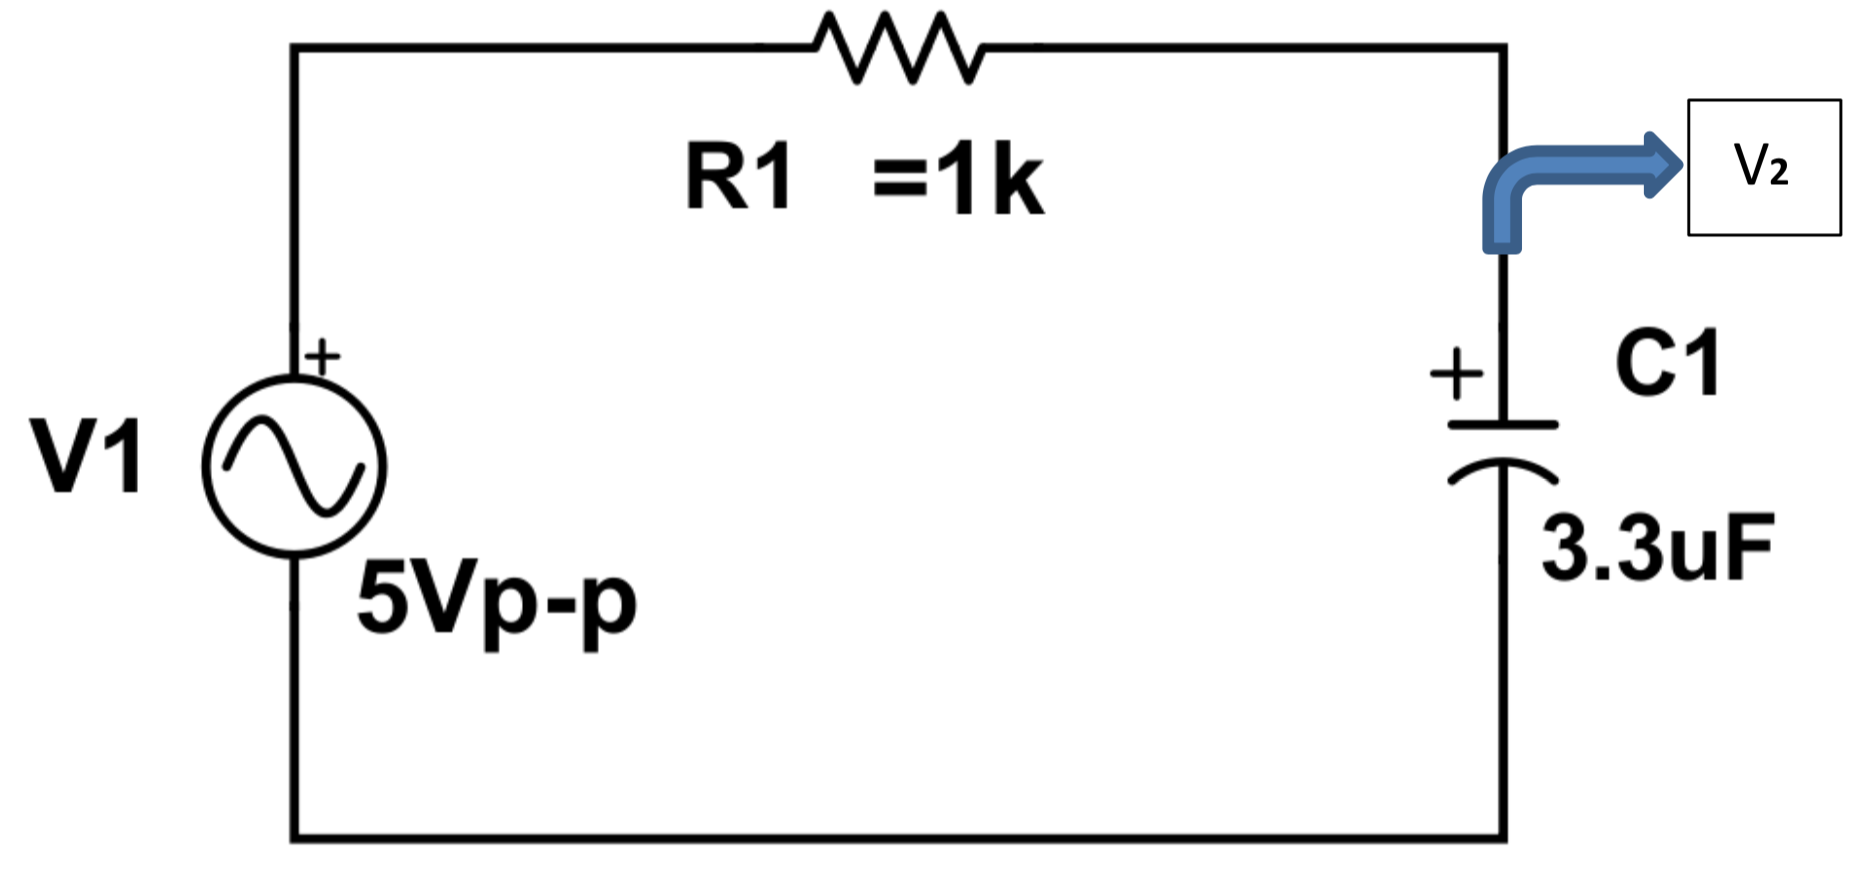
\includegraphics[width=\columnwidth]{images/lab8_circuit1.png}
    \captionof{figure}{Circuit 1}
    \label{fig:circ1}
    \medskip
\endgroup

\noindent Following the schematic above (Figure \ref{fig:circ1}), the circuit was prototyped on a breadboard. To measure the output signal, the positive terminal of the oscilloscope was attached to the leg of the capacitor, while the negative terminal to the common ground of the circuit. $R_1$ was selected to be $1k\ohm$ and the capacitor was selected to be 3.3$uF$. Once the circuit was built (see Figure \ref{fig:circ1image}), 5V p-p sinusoidal waves at 1 kHz, later 2 kHz, were applied. The phase shifts between the original sinusoidal wave and the output waveform, as well  as the magnitudes of each, were measured using the cursor functionality of the oscilloscope. Later, the frequency of the waveform was increased up to 40 kHz to observe the gradual change in the phase shift.

\bigskip

\begingroup
    \centering
    \medskip
    %width=\columnwidth
    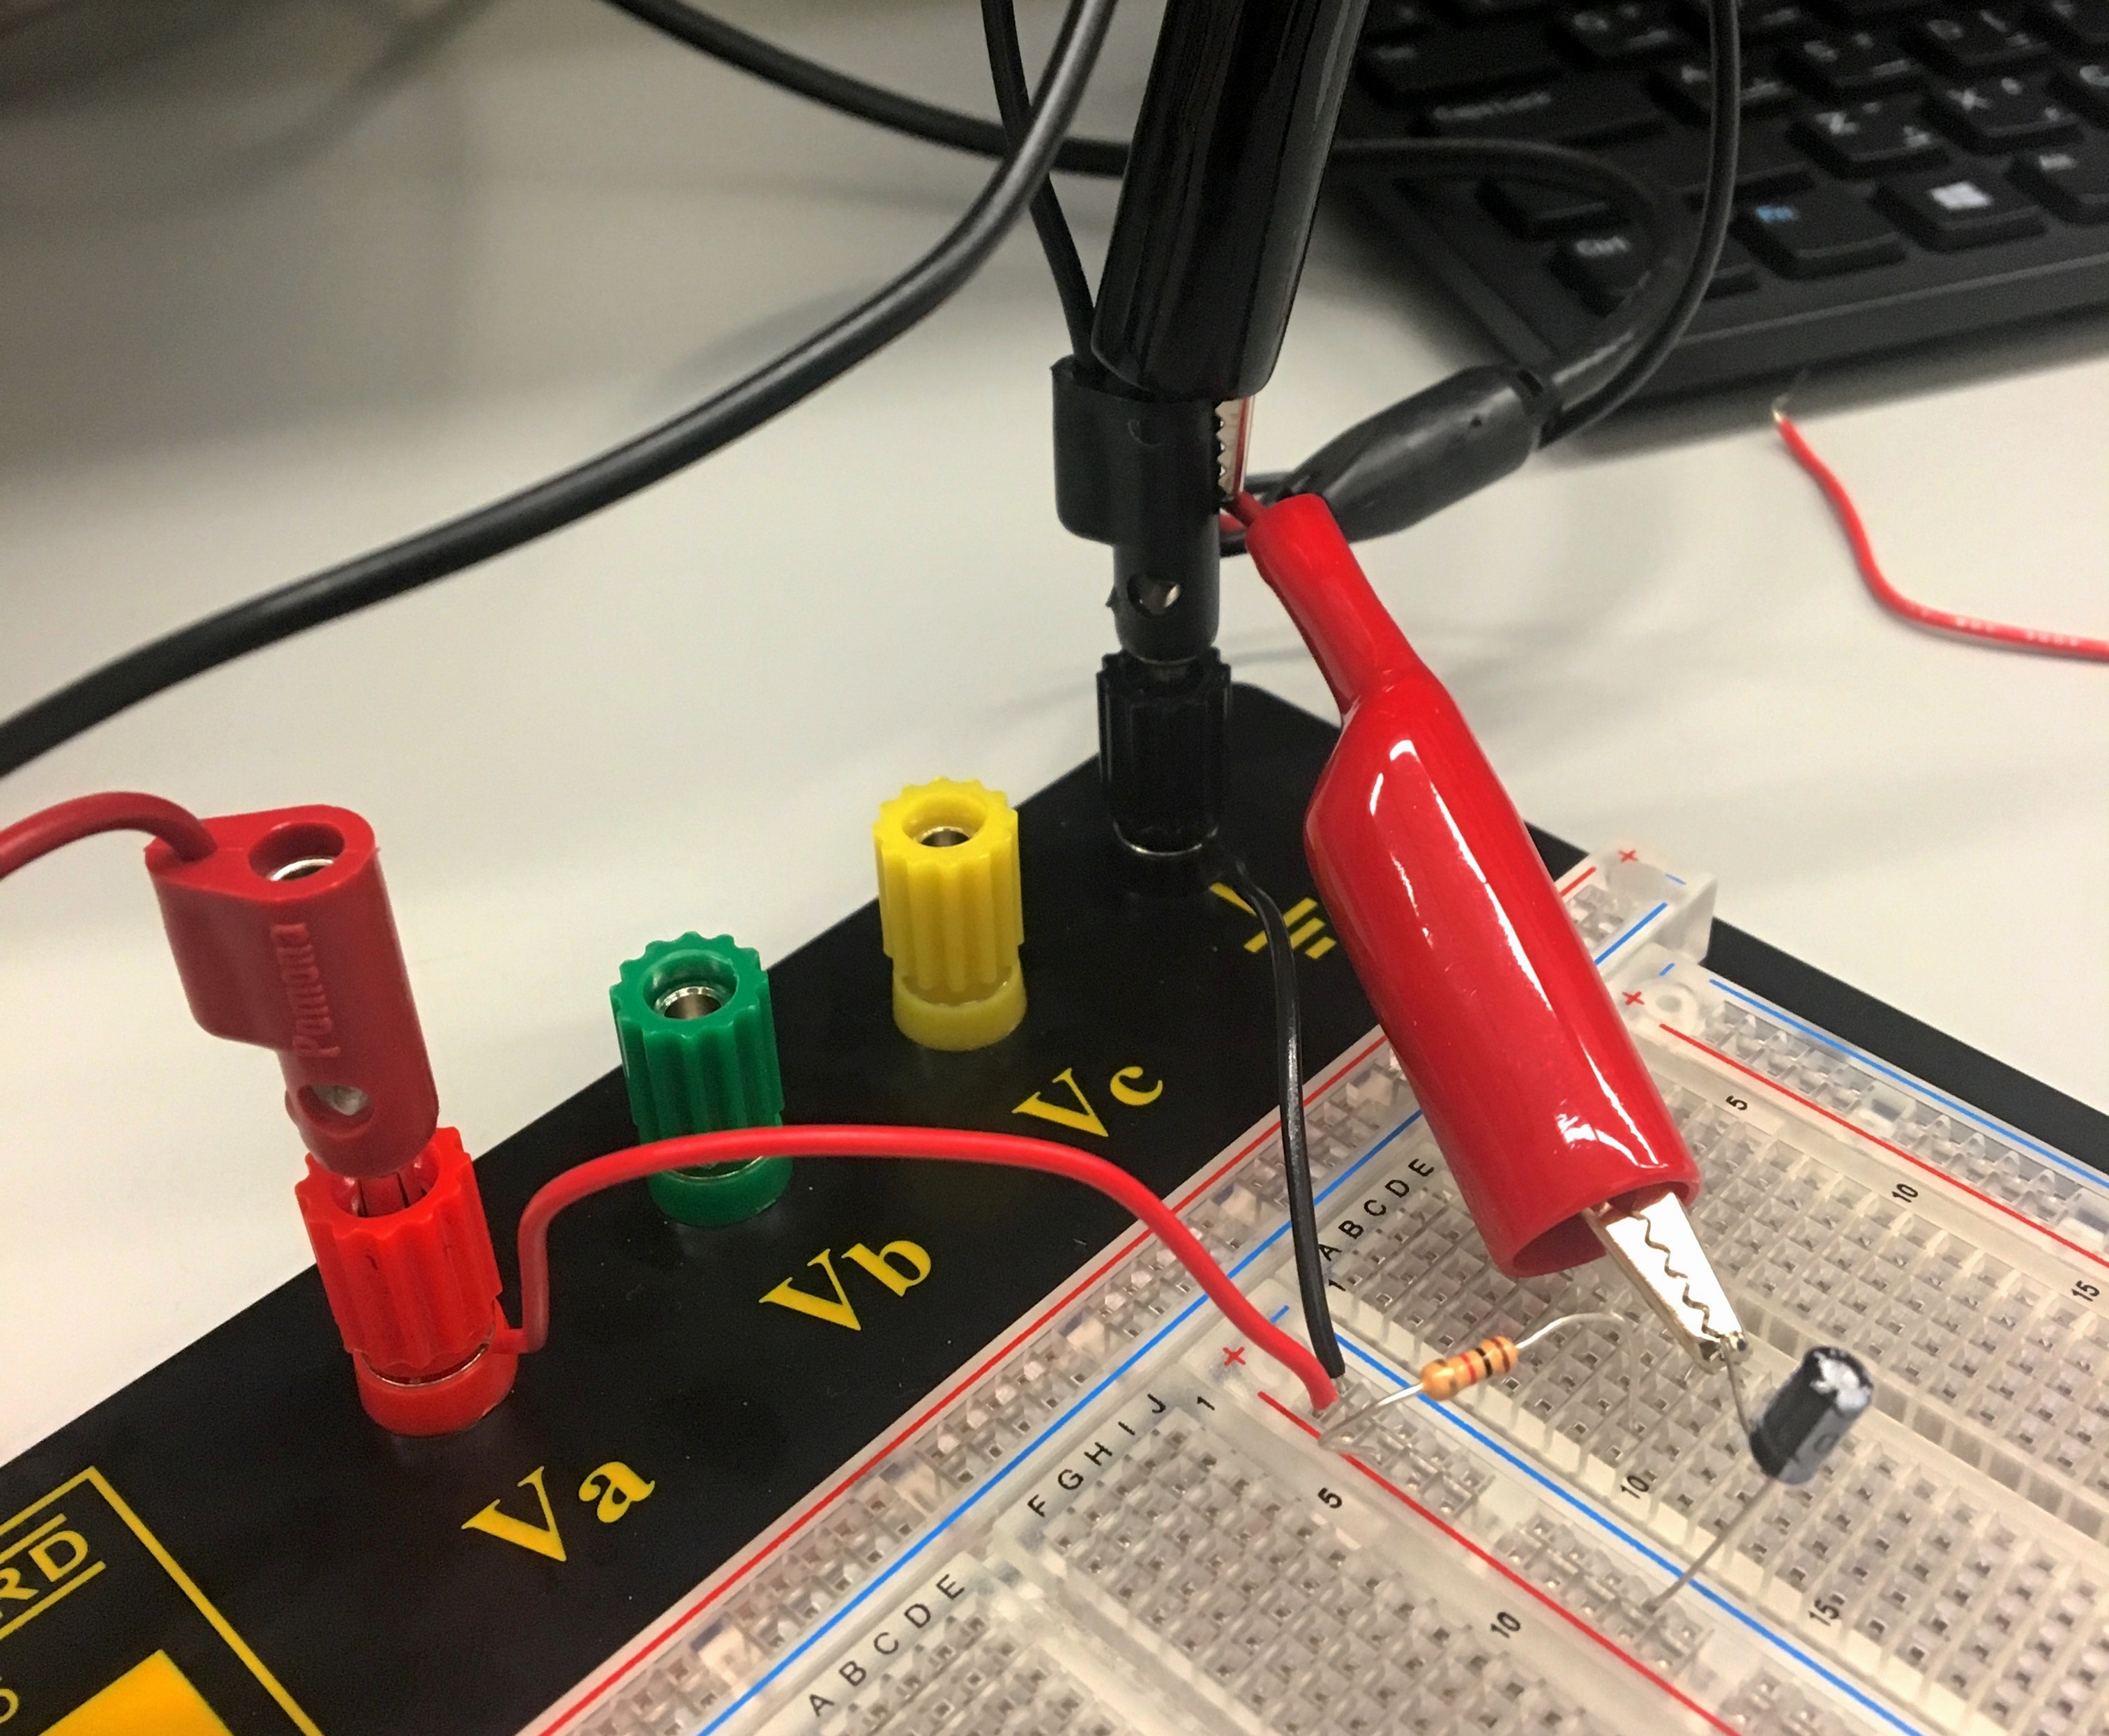
\includegraphics[width=\columnwidth]{images/lab8_circ1.jpg}
    \captionof{figure}{A RC Circuit Prototype}
    \label{fig:circ1image}
    \medskip
\endgroup



%%%%%%%%%%%%%%%%
%% RL Circuit %%
%%%%%%%%%%%%%%%%
\subsection{RL Circuit}
\noindent In a RL circuit, unlike RC circuits, voltage leads the current. Phasor diagrams depict the voltage drop across a resistor as a real vector and the voltage drop across an inductor as an imaginary vector in the positive axis. The sum of these two vectors provides an angle $\theta$, which explains the phase shift between input and output voltages.\\

\begingroup
    \centering
    \medskip
    %width=\columnwidth
    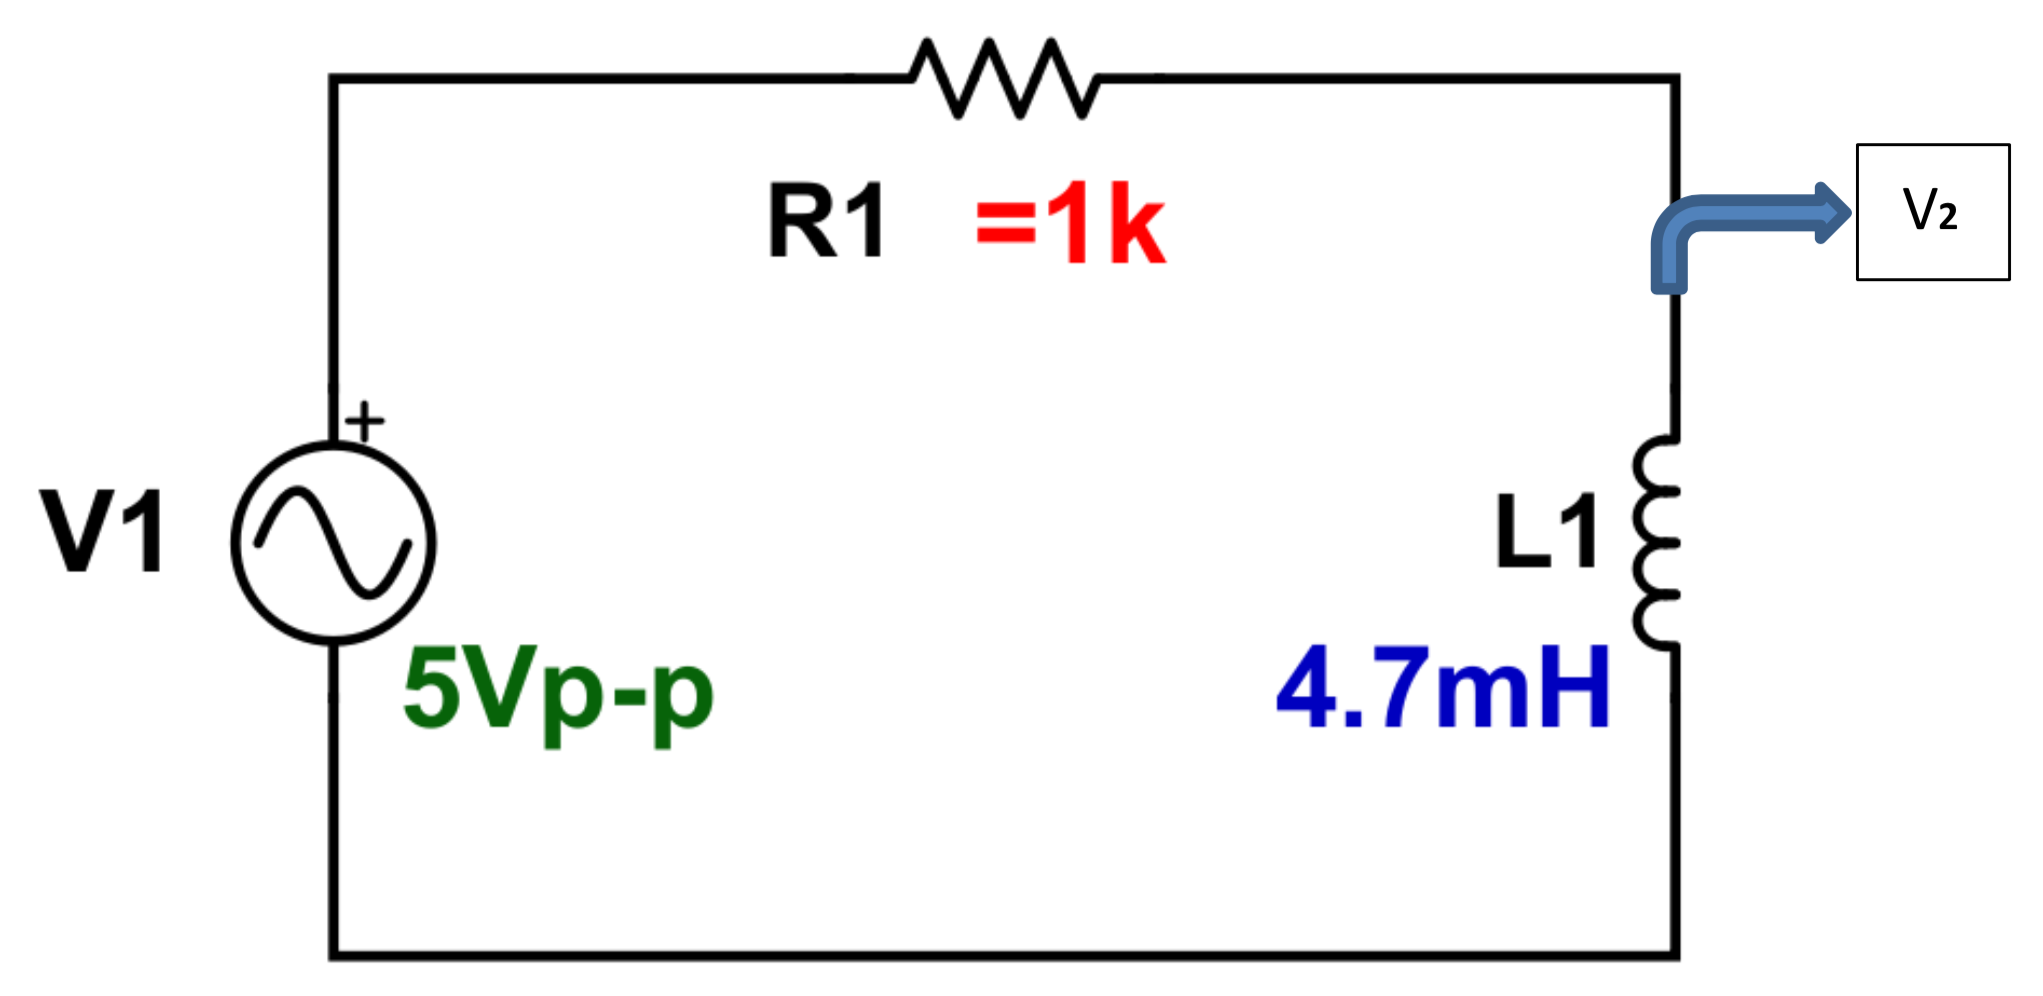
\includegraphics[width=\columnwidth]{images/lab8_circuit2.png}
    \captionof{figure}{Circuit 2}
    \label{fig:circ2}
    \medskip
\endgroup

\\
\medskip


\noindent The circuit was built following Figure \ref{fig:circ2}. The output signal was similarly measured with one crocodile grabber on the leg of an inductor and another on the common ground. One 4.7mH inductor and one 1K \ohm resistor were used in the circuit. Once the circuit was built (see Figure \ref{fig:circ2image}), the magnitude of the output voltage and the phase difference between the supplied signal and the output signal were recorded. The measurements were repeated for 1kHz and 2 kHz frequencies. \\

\begingroup
    \centering
    \medskip
    %width=\columnwidth
    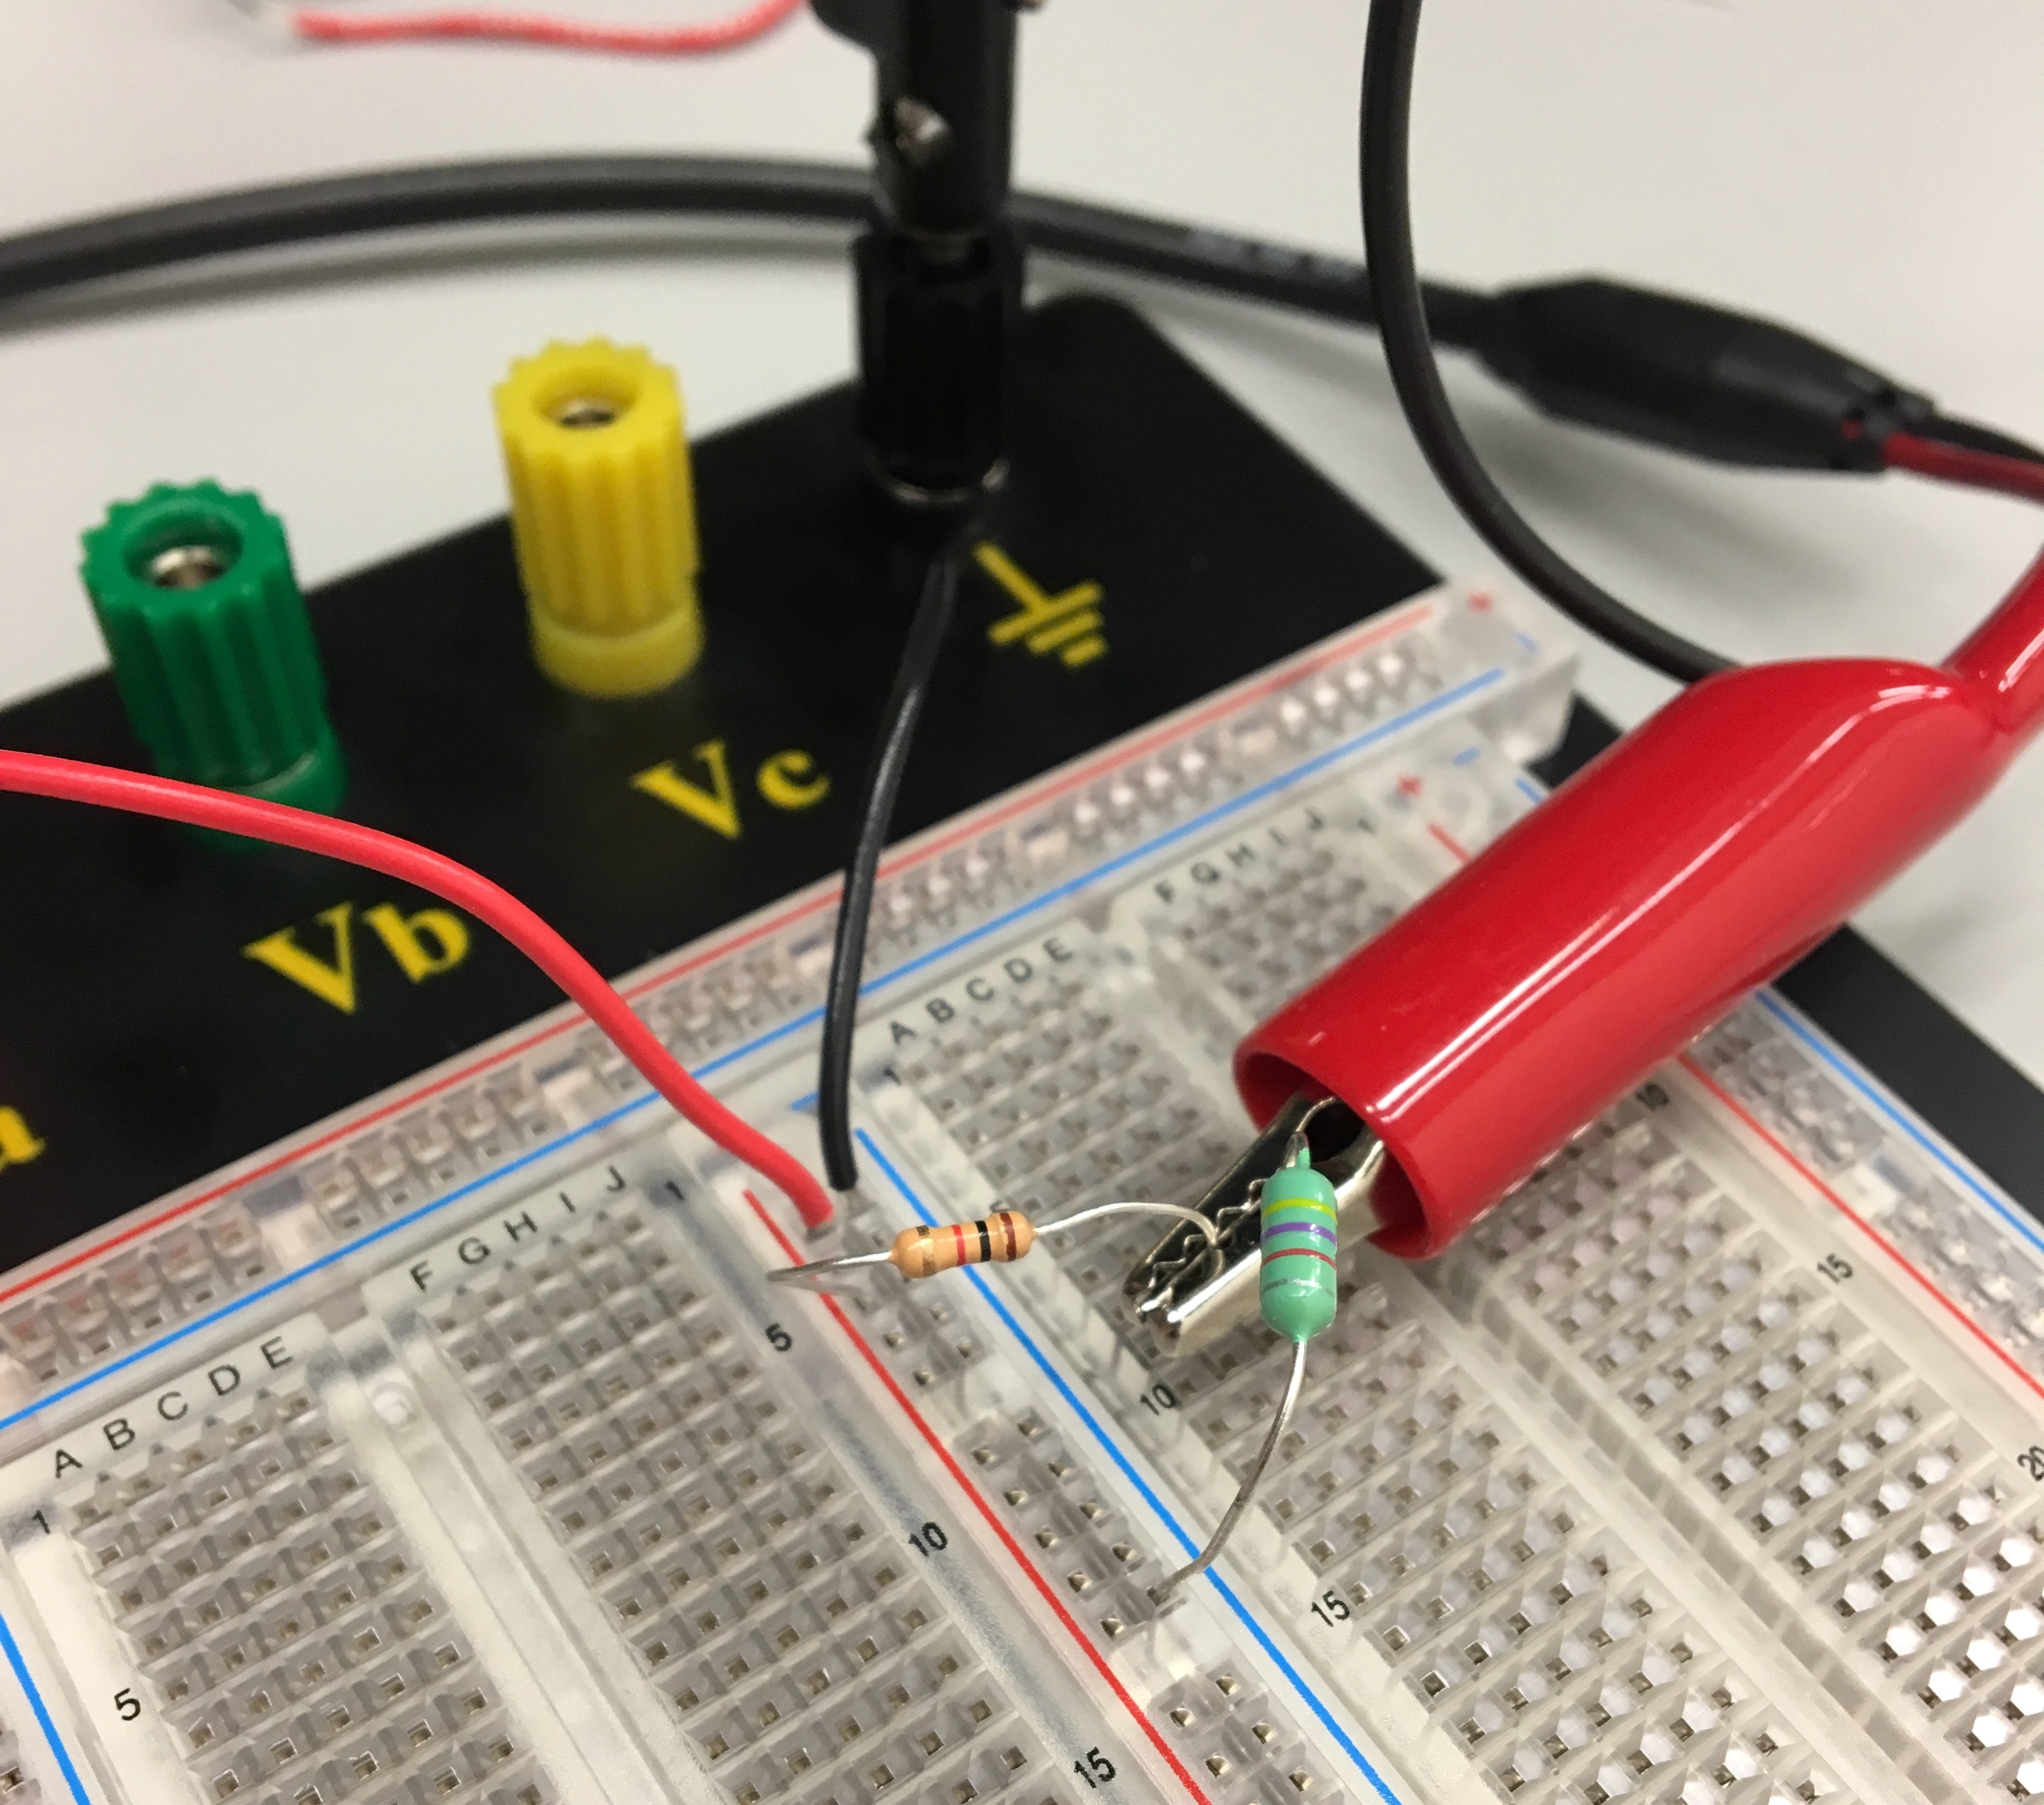
\includegraphics[width=\columnwidth]{images/lab8_circ2.jpg}
    \captionof{figure}{A RL Circuit Prototype}
    \label{fig:circ2image}
    \medskip
\endgroup



%%%%%%%%%%%%%%%%%
%% RLC Circuit %%
%%%%%%%%%%%%%%%%%
\subsection{RLC Circuit}
\noindent In a series RLC circuit, there is no leading or lagging of current and voltage, because the imaginary current components cancel out. However, a lead or lag may or may not exist between the output and input voltage depending on the reactance of the capacitor and inductor. In a case where the reactance of the L and C are equal but opposite vectors, then the imaginary component is cancelled out and output voltage has no difference in phase. 

\begingroup
    \centering
    \medskip
    %width=\columnwidth
    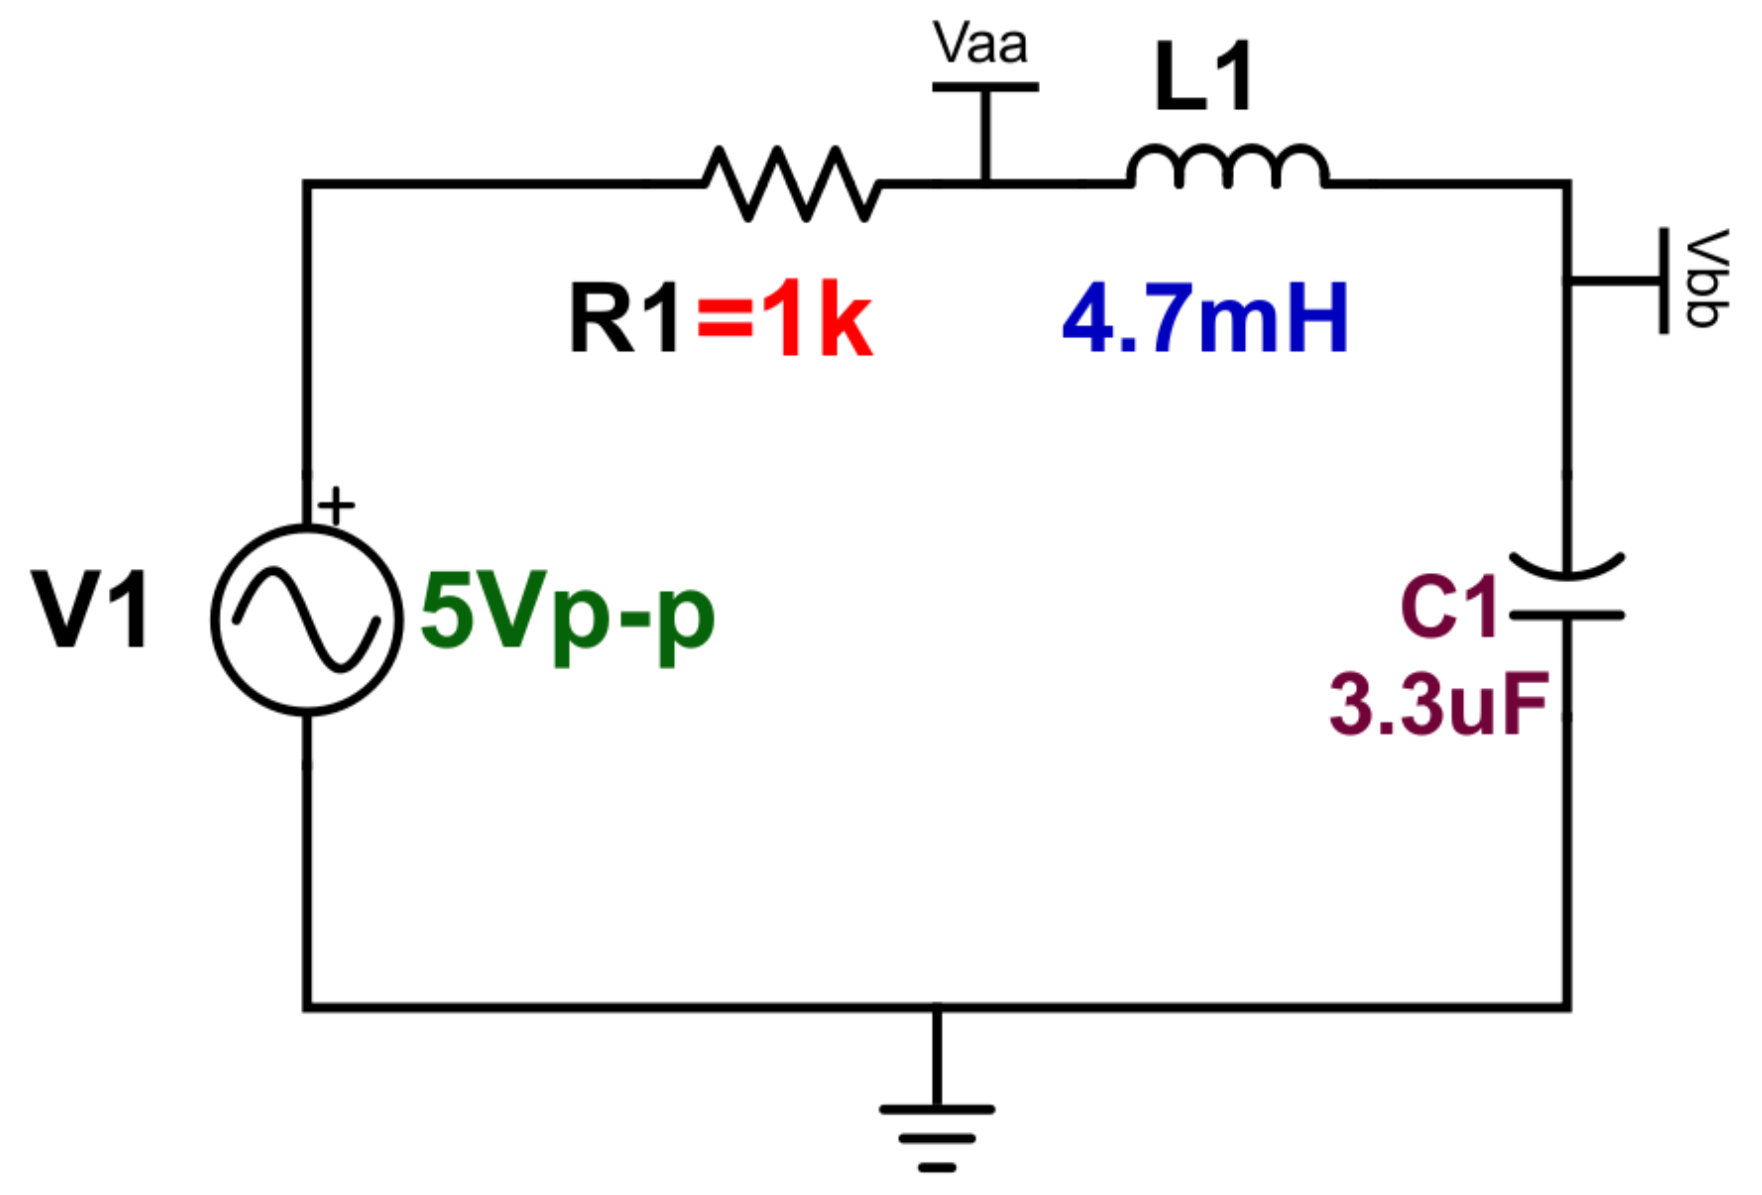
\includegraphics[width=\columnwidth]{images/lab8_circuit3.png}
    \captionof{figure}{A RLC Circuit Prototype}
    \label{fig:circ3}
    \medskip
\endgroup

\\
\medskip

\noindent The final circuit was built following Figure \ref{fig:circ3}. A 1K resistor, 4.7 $mH$ inductor, and 3.3 $uF$ capacitor were used along with the AC wave generator. In this case, two output voltages were measured. The first output signal was measured by connecting the positive terminal to the leg of the resistor adjacent to the inductor and the negative terminal to the common ground. The second output signal was measured by connecting positive terminal to the leg of the inductor adjacent to the capacitor and the negative terminal to the common ground. AC 5v p-p voltage at a frequency of 1kHz was provided as input voltage to the circuit in Figure \ref{fig:circ3image}. The frequency was also gradually increased by 10Hz and the changes in phase-shift was noted.

\\
\medskip
\medskip

\begingroup
    \centering
    \medskip
    %width=\columnwidth
    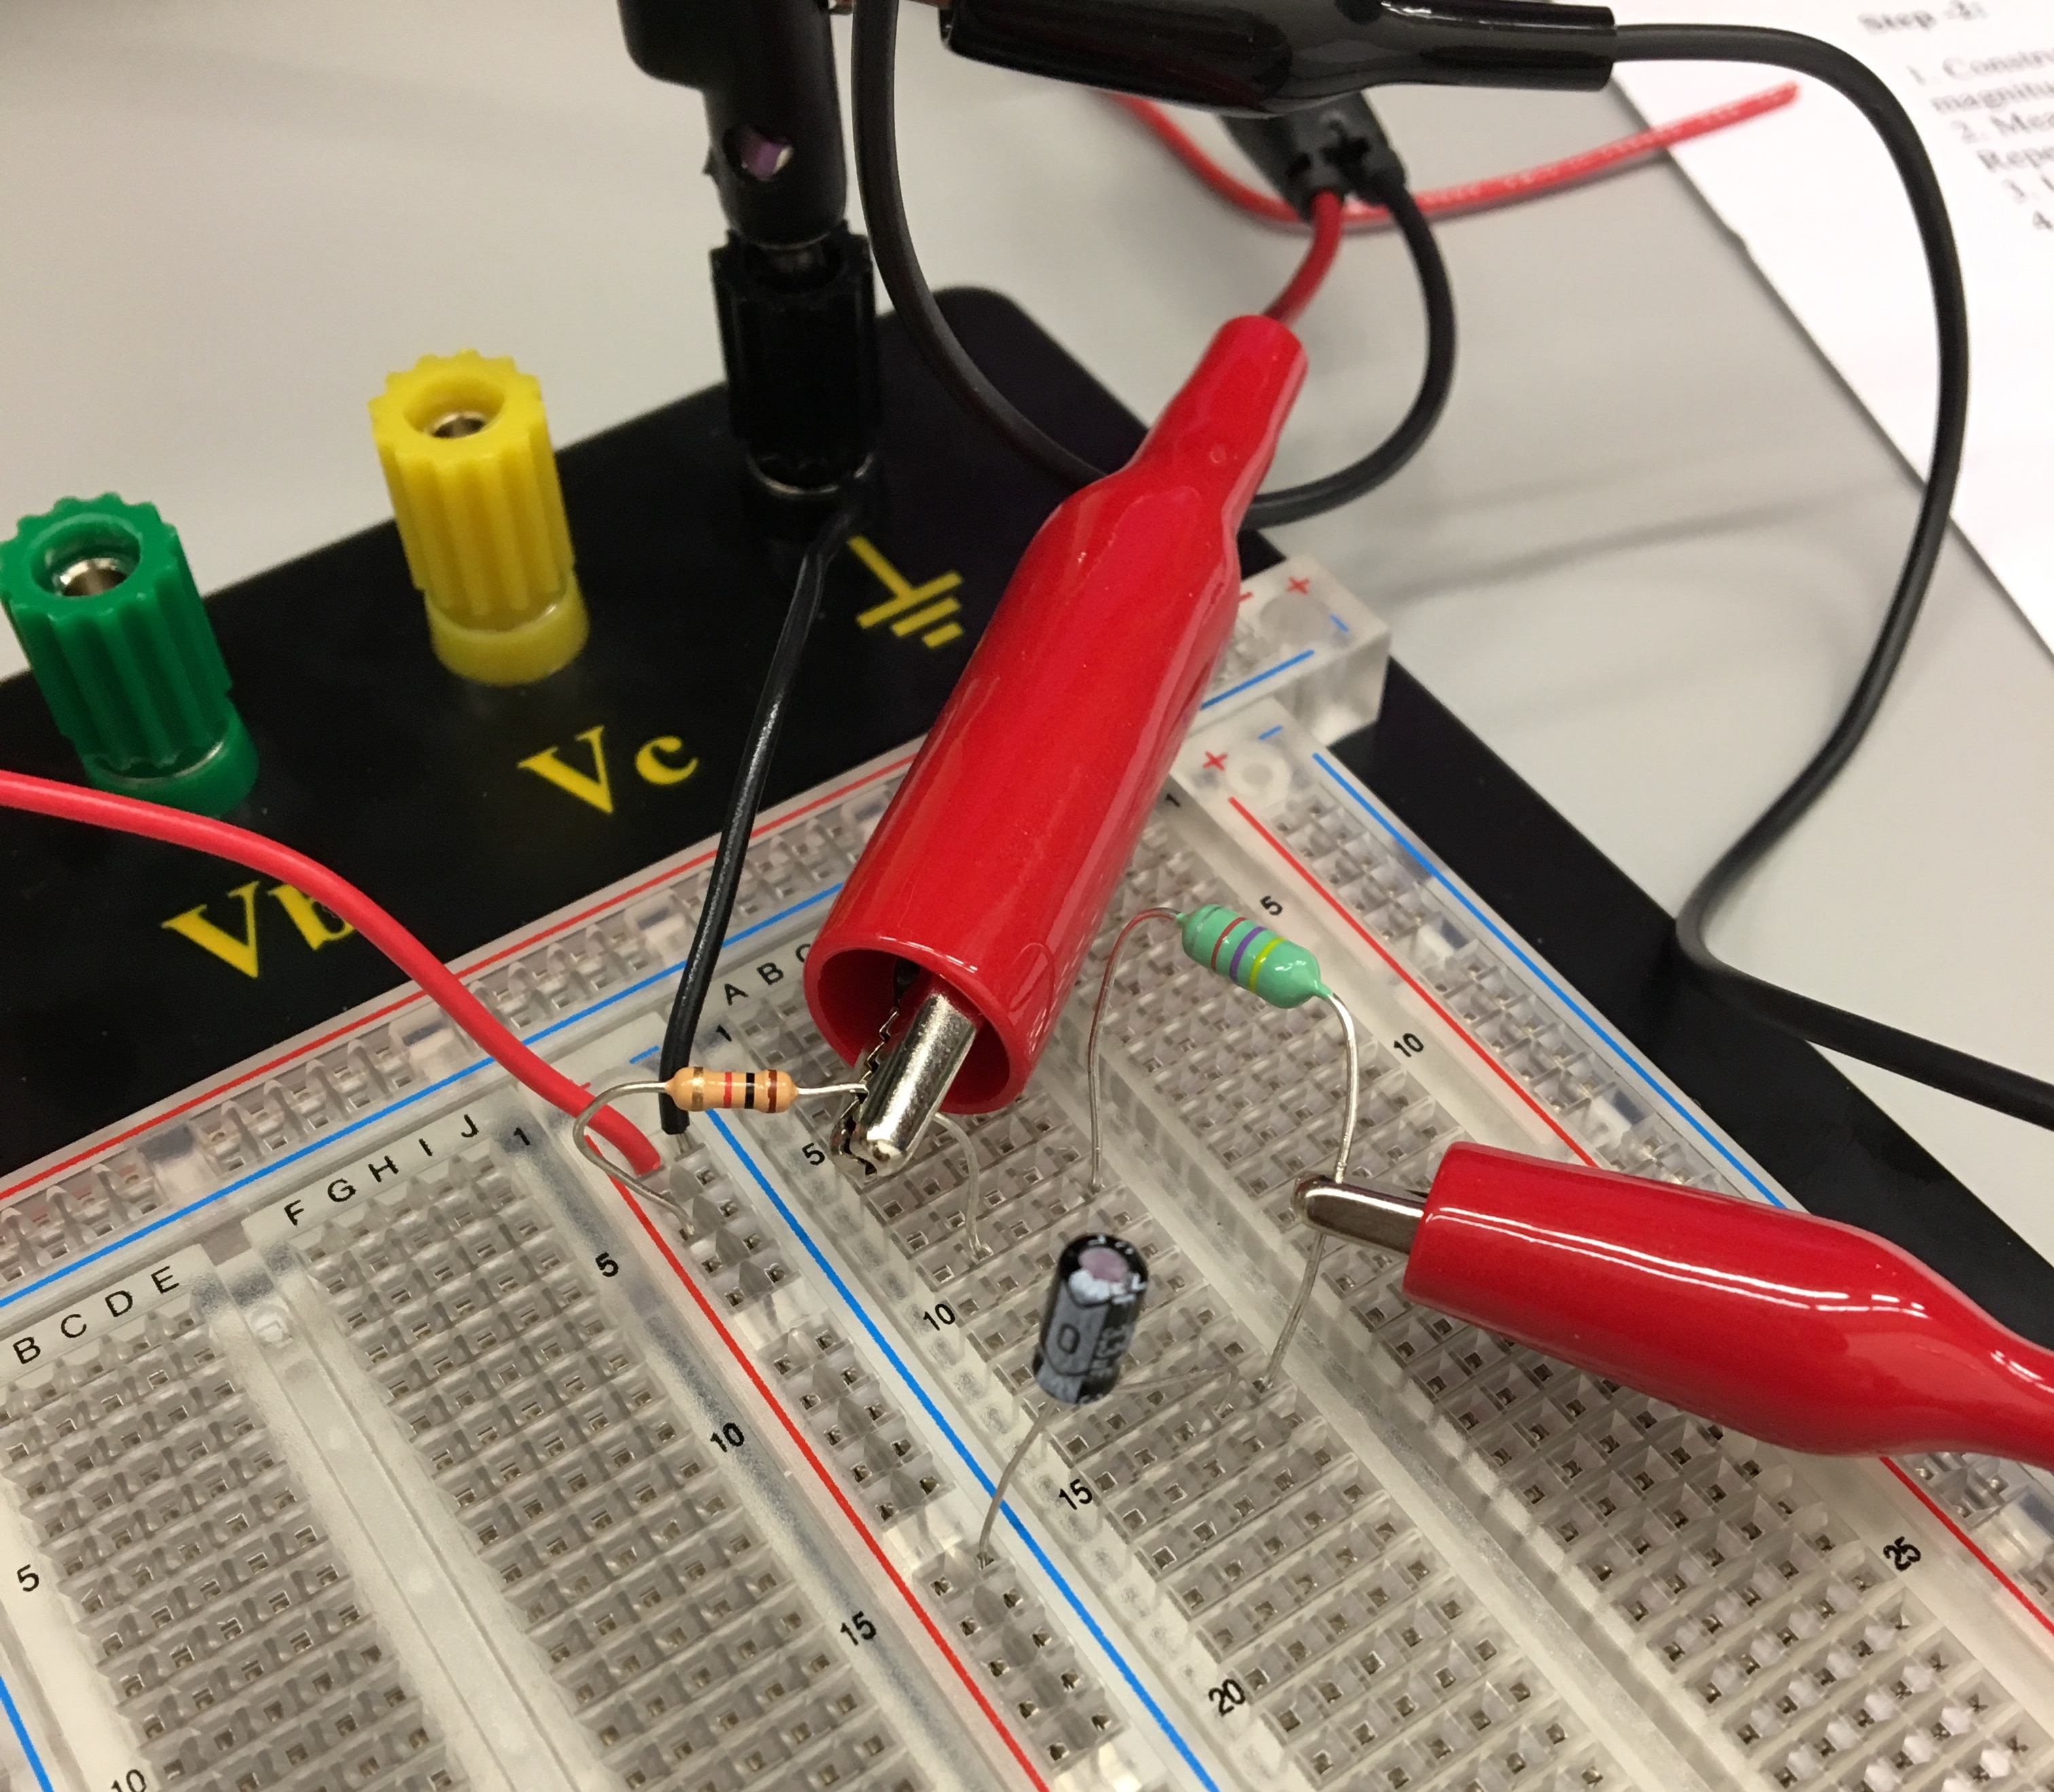
\includegraphics[width=\columnwidth]{images/lab8_circ3.jpg}
    \captionof{figure}{Circuit 3}
    \label{fig:circ3image}
    \medskip
\endgroup

\pagebreak

\section{Results and Discussion}

\noindent All configurations operated, albeit far from ideal scenarios, and the results of each circuit configuration were recorded in tables and the observed wave forms were captured. Green lines represents the signal directly coming from the AC function generator and yellow and purple lines represent the signal captured from the reactive components of the circuit.

%%%%%%%%%%%%%%%%
%% RC Circuit %%
%%%%%%%%%%%%%%%%
\subsection{RC Circuit}
\noindent Equation \ref{eq:cap_reactance} shows the calculated reactance of the capacitor, assuming a 1kHz signal.

\begin{equation}
Z_{C} = \frac{1}{2\pi fcj} = \frac{1}{2\pi(1\cdot10^3)(3.3\cdot10^{-6})j} = 0 - 48.25j
\label{eq:cap_reactance}
\end{equation}
\\

\noindent Therefore, the impedance is $1000\ohm - 48.25j\ohm$. When written in polar form, it is $1001.16 \angle-2.76\degree$. The equation \ref{eq:calcRC} depicts the calculations needed to obtain the phase angle of the voltage across the capacitor, $V_{c}$. Simply, the current is obtained by dividing the voltage by the circuit's impedance. The obtained current is then multiplied by the capacitor's reactance to obtain the phase angle of $V_c$.

\begin{equation}
    \begin{split}
        V_s & = I \angle \alpha \times Z \angle \beta \\
        0 & = \alpha - 2.76 \\
        \alpha & = 2.76 
    \end{split}
    \label{eq:calcRC}
\end{equation} \\

\noindent The expected current and output voltage can also be calculated for each frequency. Equations \ref{eq:calcRCcurrent} and \ref{eq:calcRC2} show the process for 1kHz. 

  
        
\begin{equation}
    \begin{split}
        I \angle \alpha & = \frac{V_s}{Z \angle \beta} \\
        I \angle \alpha & = \frac{5 \angle 0}{1001.16 \angle -2.76}\\
        I \angle \alpha & = 0.005 \angle 2.76 \ A\\
    \end{split}
    \label{eq:calcRCcurrent}
\end{equation} \\

\noindent Here, the reactance $0 - 48.25j$ of the capacitor, calculated in Equation \ref{eq:cap_reactance}, was converted into the polar form. This provided the polar angle of the reactance, which was $-90\degree$. This angle value was used in Equation \ref{eq:calcRC2} to calculate the output voltage magnitude and phase difference. \\

\begin{equation}
    \begin{split}
        V_c & = I \angle \alpha \times X \angle 90 \\
        V_c & =  0.005 \angle 2.76 \times 48.25 \angle -90 \\
        V_c & = 0.241 \angle -87.24 V \\
    \end{split}
    \label{eq:calcRC2}
\end{equation} \\

\noindent Calculations (\ref{eq:cap_reactance}, \ref{eq:calcRC}, and \ref{eq:calcRC2}) were repeated for 2 kHz AC source voltage and results were recorded in Table \ref{fig:rctable2}.

\small
    \begingroup
    \bigskip
        \centering
        \def\arraystretch{1.5}
        \setlength\tabcolsep{3pt}
            \begin{tabular}{ccccccc}
                \toprule
                    \thead{Frequency\\(kHz)} & \thead{Vin\\(V)} & \thead{Impedance\\(\ohm)} &\thead{Calculated \\ Vout\\(mV)} & \thead{Calculated \\ Phase\\Difference\\(\degree)} & \thead{Calculated \\ Current \\ (mA)}\\
                \midrule
                    1 & 5 & 1000 - 48.25j & 241 & -87.24 & 5\\
                    2 & 5 & 1000 - 24.13j & 121 & -88.62 & 5\\
                \bottomrule
            \end{tabular}
        \captionof{figure}{Tabulation of the calculations for the built RC circuit }
        \label{fig:rctable}
    \endgroup
\normalsize


\small
    \begingroup
    \bigskip
        \centering
        \def\arraystretch{1.5}
        \setlength\tabcolsep{3pt}
            \begin{tabular}{ccccccc}
                \toprule
                   \thead{Frequency\\(kHz)} & \thead{Vin\\(V)} & \thead{Impedance\\(\ohm)} &\thead{Observed \\ Vout\\(mV)} & \thead{Observed \\ Phase\\Difference\\(\degree)} & \thead{Observed \\ Current \\ (mA)}\\
                \midrule
                    1 & 5 & 1000 - 48.25j & 254  & -74 & 5\\
                    2 & 5 & 1000 - 24.13j & 150  & -72 & 5\\
                \bottomrule
            \end{tabular}
        \captionof{figure}{Tabulation of the measurements for the built RC circuit}
        \label{fig:rctable2}
    \medskip
    \endgroup
\normalsize

\noindent There were noticeable difference between the theoretical and measured phase differences and output voltages in the RC circuit. The most reasonable explanation is that the capacitor was assumed to behave ideally in the calculations, whereas in practice, its performance was hindered. As seen in Figure \ref{fig:rcosc1} and \ref{fig:rcosc2}, the output signal, in yellow, has a lower voltage than the input voltage; when looking at Figure \ref{fig:rctable}, this decrease in output voltage can explained by the lower impedance caused by the higher input frequency.


\begingroup
    \centering
    \medskip
    %width=\columnwidth
    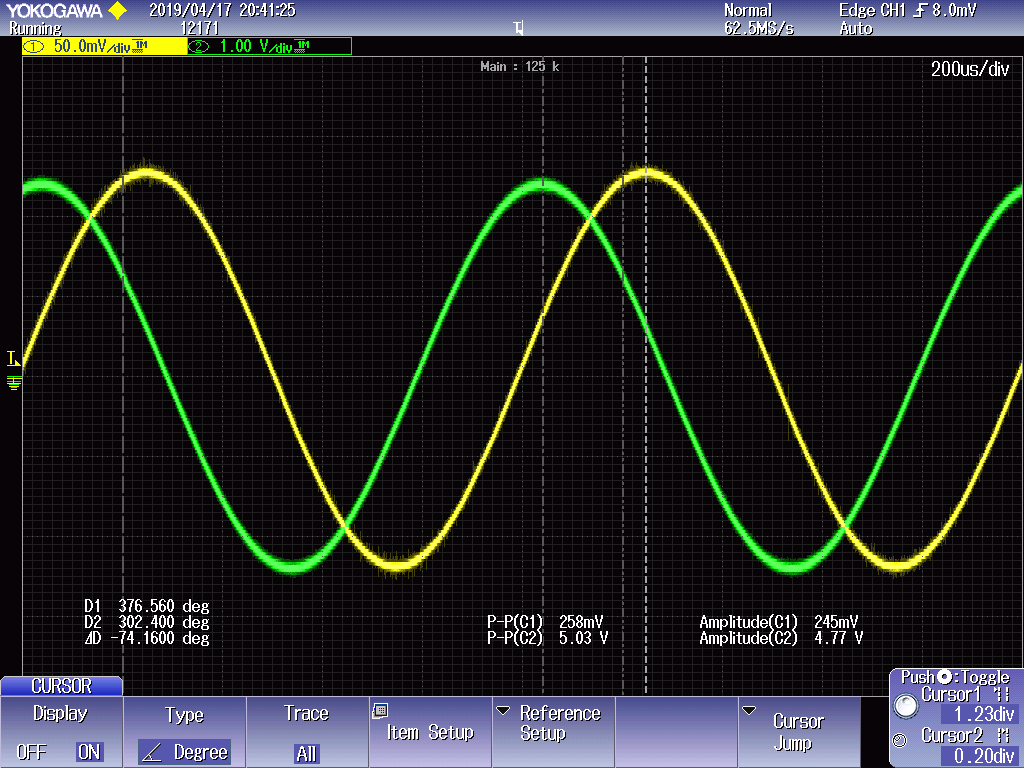
\includegraphics[width=\columnwidth]{images/lab8_002.png}
    \captionof{figure}{Phase shift of the RC circuit at 1 kHz}
    \label{fig:rcosc1}
    \medskip
\endgroup

\begingroup
    \centering
    \medskip
    %width=\columnwidth
    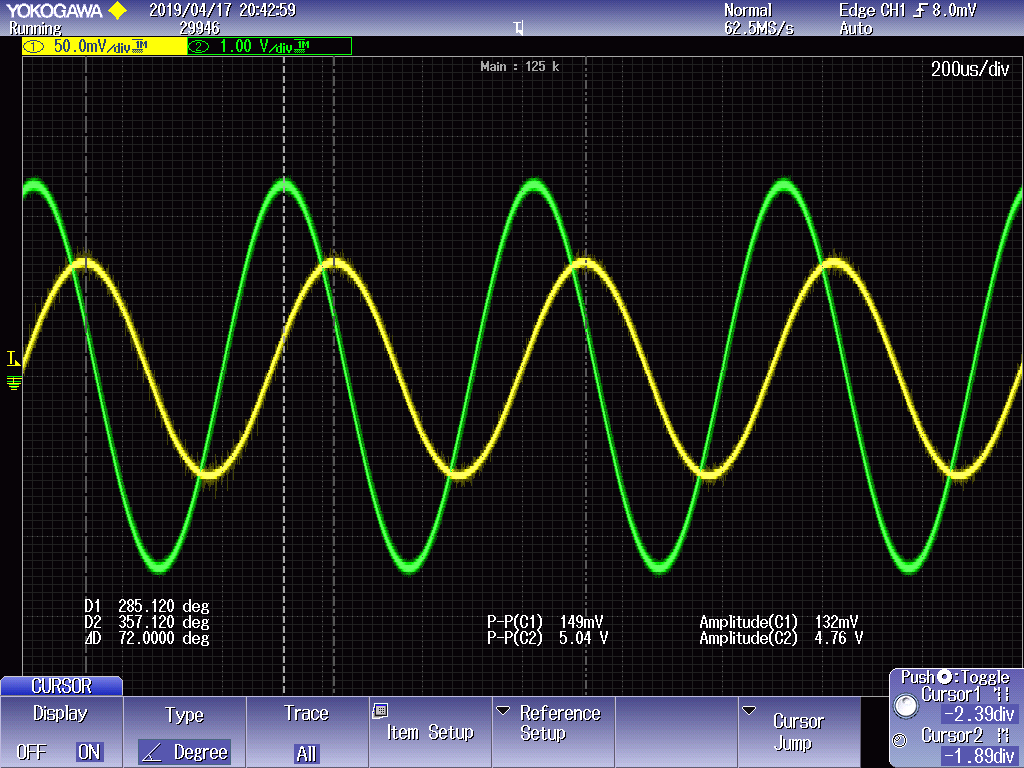
\includegraphics[width=\columnwidth]{images/lab8_005.png}
    \captionof{figure}{Phase shift of the RC circuit at 2 kHz}
    \label{fig:rcosc2}
    \medskip
\endgroup


%%%%%%%%%%%%%%%%
%% RL Circuit %%
%%%%%%%%%%%%%%%%
\subsection{RL Circuit}
\noindent Equation \ref{eq:inductor_impedance} calculates the reactance of the inductor with assumption of a 1kHz signal.

\begin{equation}
Z_{L} = 2\pi\cdot fLj = 2\pi \cdot (1\cdot10^3)(4.7\cdot10^-3)(j) = 0 + 20.72j
\label{eq:inductor_impedance}
\end{equation} \\

\noindent As before, the impedance of the circuit is then $1000\ohm + 20.72j$, which is equivalent to $1000.21 \angle1.19\degree$. Equation \ref{eq:calcRL} shows the calculations to obtain phase angle of ${V_L}$. Current of the circuit is obtained by dividing voltage by impedance; this current is then multiplied by the inductor's reactance to obtain the phasor angle of ${V_L}$. \\

\begin{equation}
    \begin{split}
        V_s & = I \angle \alpha \times Z \angle \beta \\
        0 & = \alpha + 1.19 \\
        \alpha & = -1.19
    \end{split}
    \label{eq:calcRL}
\end{equation} \\

\noindent The expected current and output voltage can also be calculated for each frequency. Equations \ref{eq:calcRCcurrent} and \ref{eq:calcRL2} show the process for 1kHz.

\begin{equation}
    \begin{split}
        I \angle \alpha & = \frac{V_s}{Z \angle \beta} \\
        I \angle \alpha & = \frac{5 \angle 0}{1000.2 \angle 1.19}\\
        I \angle \alpha & = 0.005 \angle -1.19 \ A\\
    \end{split}
    \label{eq:calcRCcurrent}
\end{equation} \\

\noindent The reactance of the inductor,  $0 + 20.72j$, is once again rewritten in polar form. Converted angle value was used in Equation \ref{eq:calcRL} to calculate the phase difference as shown in Equation \ref{eq:calcRL2}.

\begin{equation}
    \begin{split}
        V_l & = I \angle \alpha \times X \angle 90 \\
        V_l & =  0.005 \angle 2.76 \times 20.72 \angle 90 \\
        V_l & = 0.104 \angle 88.81 V \\
    \end{split}
    \label{eq:calcRL2}
\end{equation} \\

\noindent The calculations shown above were repeated for a 2kHz input signal, with all measurements recorded in Table \ref{fig:rltable2}.


\small
    \begingroup
    \bigskip
        \centering
        \def\arraystretch{1.5}
        \setlength\tabcolsep{3pt}
            \begin{tabular}{ccccccc}
                \toprule
                    \thead{Frequency\\(kHz)} & \thead{Vin\\(V)} & \thead{Impedance\\(\ohm)} &\thead{Calculated \\ Vout\\(mV)} & \thead{Calculated \\ Phase\\Difference\\(\degree)} & \thead{Calculated \\ Current \\ (mA)}\\
                \midrule
                    1 & 5 & 1000 + 20.72j & 104 &  88.81  & 5\\
                    2 & 5 & 1000 + 10.36j & 52 &  89.1   & 5\\
                \bottomrule
            \end{tabular}
        \captionof{figure}{Tabulation of the calculations for the built RL circuit}
        \label{fig:rltable}
    \medskip
    \endgroup
\normalsize

\small
    \begingroup
    \bigskip
        \centering
        \def\arraystretch{1.5}
        \setlength\tabcolsep{3pt}
            \begin{tabular}{ccccccc}
                \toprule
                    \thead{Frequency\\(kHz)} & \thead{Vin\\(V)} & \thead{Impedance\\(\ohm)} &\thead{Observed \\ Vout\\(mV)} & \thead{Observed \\ Phase\\Difference\\(\degree)} & \thead{Observed \\ Current \\ (mA)}\\
                \midrule
                    1 & 5 & 1000 + 20.72j & 220 &  40  & N/A\\
                    2 & 5 & 1000 + 10.36j & 320 &  50   & N/A\\
                \bottomrule
            \end{tabular}
        \captionof{figure}{Tabulation of the measurements
        for the built RL circuit}
        \label{fig:rltable2}
    \medskip
    \endgroup
\normalsize



\noindent In this case, there was a significant difference between the expected and measured phase difference. The most likely explanation is the lack of precision in the inductor value and its relatively low quality. Figure \ref{fig:rlosc1} and \ref{fig:rlosc2} show the output voltage at a higher voltage, which is explained by the higher impedance caused by the increase in frequency.

\begingroup
    \centering
    \medskip
    %width=\columnwidth
    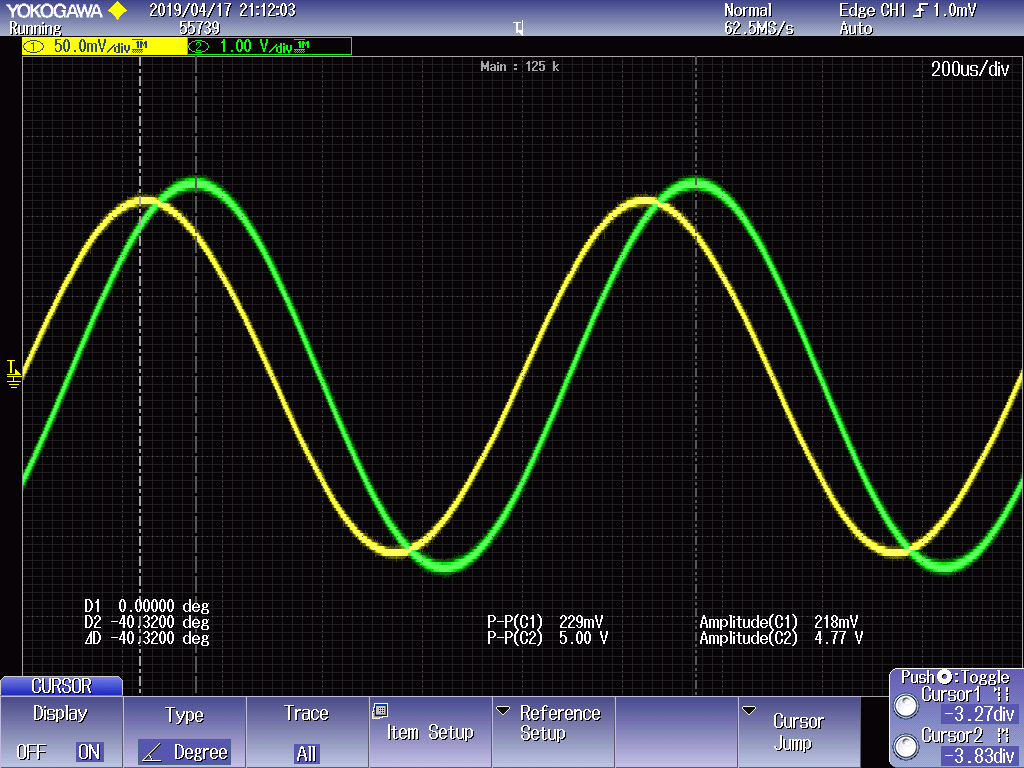
\includegraphics[width=\columnwidth]{images/lab8_014.png}
    \captionof{figure}{Phase shift of the RL circuit at 1 kHz}
    \label{fig:rlosc1}
    \medskip
\endgroup

\begingroup
    \centering
    \medskip
    %width=\columnwidth
    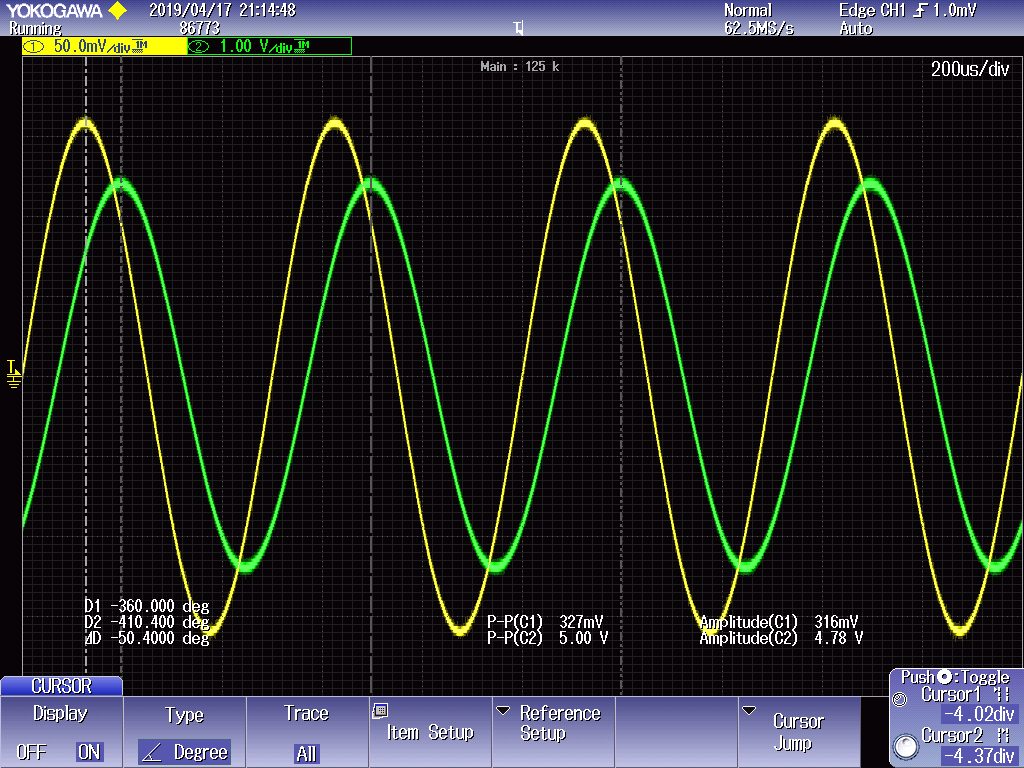
\includegraphics[width=\columnwidth]{images/lab8_017.png}
    \captionof{figure}{Phase shift of the RL circuit at 2 kHz}
    \label{fig:rlosc2}
    \medskip
\endgroup


%%%%%%%%%%%%%%%%%
%% RLC Circuit %%
%%%%%%%%%%%%%%%%%
\subsection{RLC Circuit}
Equation \ref{eq:rlcimpedance} calculates the total impedance of the RLC circuit.\\


% Z_{RLC} = = 999.83+(-18.67j)
\begin{equation}
    \begin{split}
        Z_{C} & = \frac{1}{2\pi fcj} = \frac{1}{2\pi(1\cdot10^3)(3.3\cdot10^{-6})j} = 0 - 48.25j \\ 
        Z_{L} & = 2\pi\cdot fLj = 2\pi \cdot (1\cdot10^3)(4.7\cdot10^-3)(j) = 0 + 20.72j \\
        Z_{R} & = 1000 + 0j \\ 
        \\
        Z_{RLC} & = -48.25j + 20.72j + 1000\\
                & = 1000 - 27.5j
    \end{split}
    \label{eq:rlcimpedance}
\end{equation} \\

\noindent Rewritten in polar form, the equation is equivalent to $1000.17 \angle-1.58\degree$. As seen before, a negative angle implies that the system is capacitive. Therefore, we can infer that the output voltage leads the input voltage, as was in the case of the RC circuit. Looking at the measurements in Table \ref{fig:rlctable}, it is clear that the phase difference is negative, hence the output voltage does in fact lead the input voltage. 


\begingroup
\bigskip
    \centering
    \def\arraystretch{1.5}
    \begin{tabular}{cccccc}
        \toprule
        \thead{Output} & \thead{Frequency\\(kHz)} & \thead{Vin\\(V)} & \thead{Vout\\(mV)} &\thead{Observed \\ Phase \\ Difference \\ (\degree)} \\
        \midrule
        Vaa & 1 & 5 & 260 & -20\\
        Vbb & 1 & 5 & 250 & -72\\
        \bottomrule
    \end{tabular}
    \captionof{figure}{Tabulation of the measurements for the RLC circuit built with 1K\ohm \, resistor, 4.7$mH$ inductor, and 3.3$uF$ capacitor}
    \label{fig:rcltable}
\medskip
\endgroup


\begingroup
    \centering
    \medskip
    %width=\columnwidth
    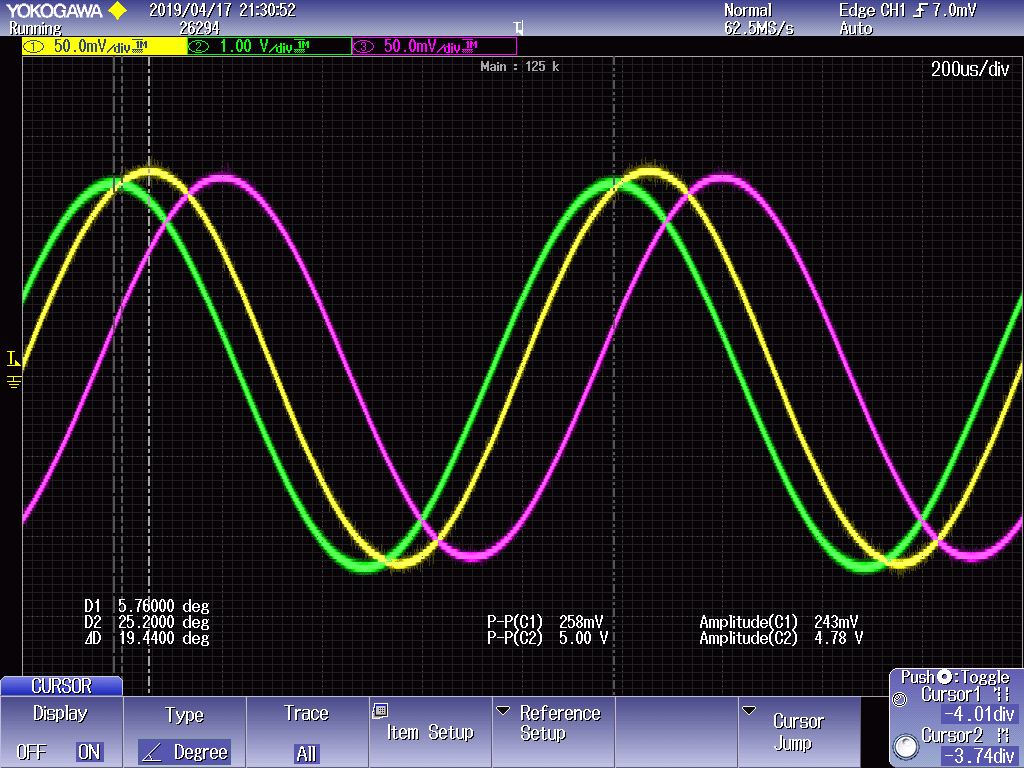
\includegraphics[width=\columnwidth]{images/lab8_025.png}
    \captionof{figure}{Phase shift of the RL circuit at 1 kHz. Yellow line represents the $V_{aa}$ while purple line represents the $V_{bb}$ signal.}
    \label{fig:rlcosc1}
    \medskip
\endgroup

\noindent As another observation, increasing the input frequency resulted in phase shifts, with a 4kHz frequency shifting the output signals behind the input signal. Comparing Figure \ref{fig:rlcosc2} and \ref{fig:rlcosc1} makes this difference obvious. This, implied the existence of a frequency at which the output signal and the input signal approximately aligned, known as resonance frequency. The resonance frequency is when the reactance of the inductor and capacitor in an RLC circuit are equal, so that the phase shifts cancel each other out. Equation \ref{eq:resfreq} shows the derivation of the formula for calculating this resonance frequency. 


    \begin{equation}
        \begin{split}
            \omega \cdot L & = Reactance \, of \, Inductor \\
            \frac{1}{\omega \cdot C} & = Reactance\, of\,  Conductor \\ 
            \omega^2 L & = \frac{1}{C}\\
            \omega^2 & = \frac{1}{LC}\\
            \omega & = \sqrt{\frac{1}{LC}}\\
            2 \pi f & = \frac{1}{\sqrt{LC}} \\
            f & = \frac{1}{2 \pi \sqrt{LC}} \\
        \end{split}
        \label{eq:resfreq}
    \end{equation} \\
    
\noindent Substituting the known values, L and C, for 4.7mH and 3.3$\mu$ F, respectively, resulted in a resonance frequency of approximately 1.28 kHz. When measured using the oscilloscope, the resonance frequency was found to be approximately 1.3 kHz (see Figure \ref{fig:phaseshift1}).



\begingroup
    \centering
    \medskip
    %width=\columnwidth
    \includegraphics[width=\columnwidth]{images/lab8_final.png}
    \captionof{figure}{Phase shift of the RL circuit at 1.3 kHz. Yellow line represents the $V_{aa}$ while purple line represents the $V_{bb}$ signal.}
    \label{fig:phaseshift1}
    \medskip
\endgroup



\begingroup
    \centering
    \medskip
    %width=\columnwidth
    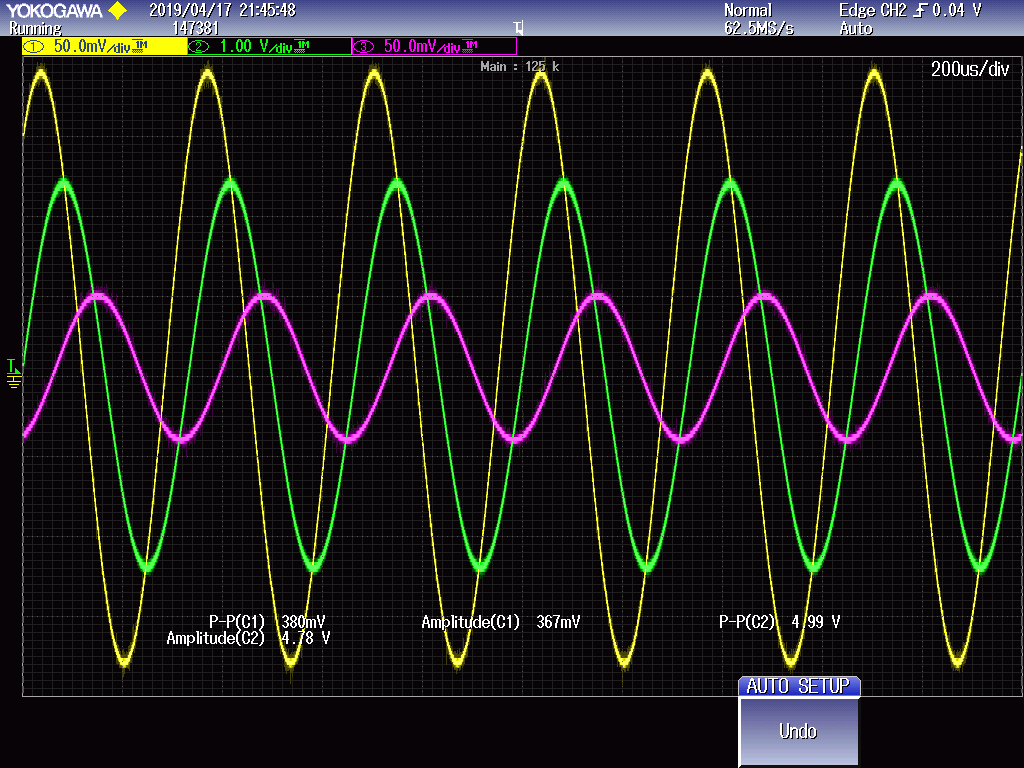
\includegraphics[width=\columnwidth]{images/lab8_029.png}
    \captionof{figure}{Phase shift of the RL circuit at 4 kHz. Yellow line represents the $V_{aa}$ while purple line represents the $V_{bb}$ signal.}
    \label{fig:rlcosc2}
    \medskip
\endgroup

%%%%%%%%%%%%%%%%%%%%%%%%%%
%% General Observations %%
%%%%%%%%%%%%%%%%%%%%%%%%%%
\subsection{General Observations}

\noindent In the case of the RC circuit, the frequency of the input signal was gradually increased until 40kHz. Figure \ref{fig:phaseshift1} shows the state of the phase shift at 1kHz and Figure \ref{fig:phaseshift40} shows the final state at 40kHz. In both images, the green signal represents the input voltage and the yellow represents the output voltage. It is clear that the output signal shifts leftwards, to eventually be in phase with the input signal. This confirms the notion that capacitors act like short circuits at high frequency signals, as impedance approaches zero.  \\


\begingroup
    \centering
    \medskip
    %width=\columnwidth
    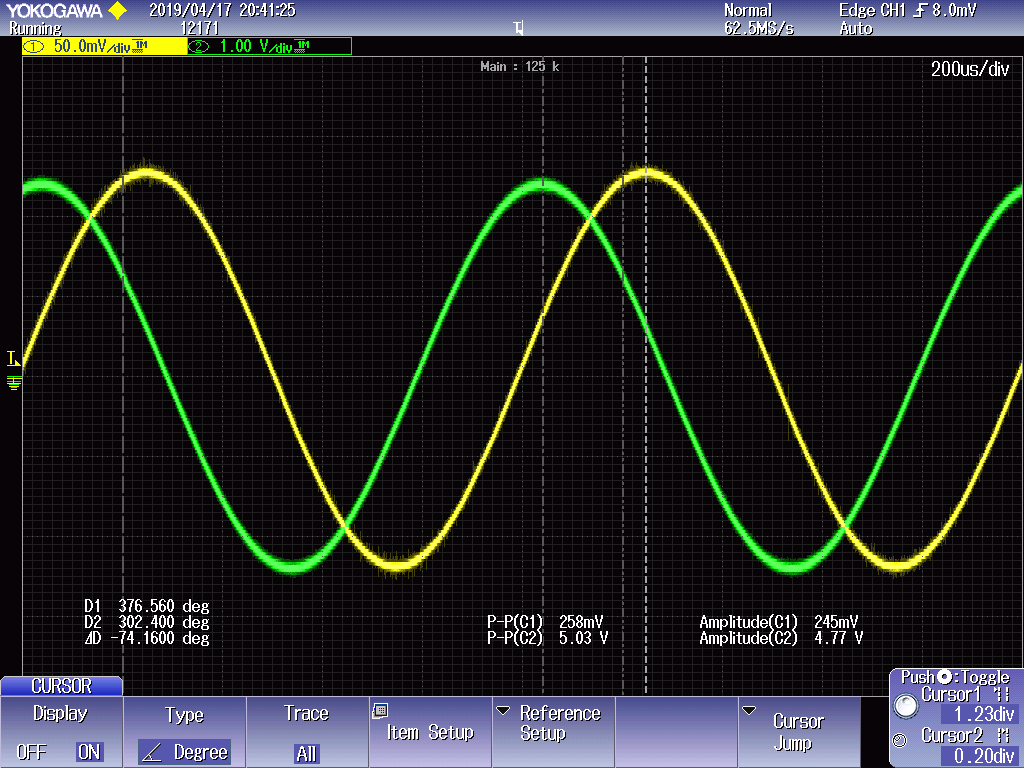
\includegraphics[width=\columnwidth]{images/lab8_002.png}
    \captionof{figure}{Phase shift at 1 kHz for the RC circuit}
    \label{fig:phaseshift1}
    \medskip
\endgroup

\begingroup
    \centering
    \medskip
    %width=\columnwidth
    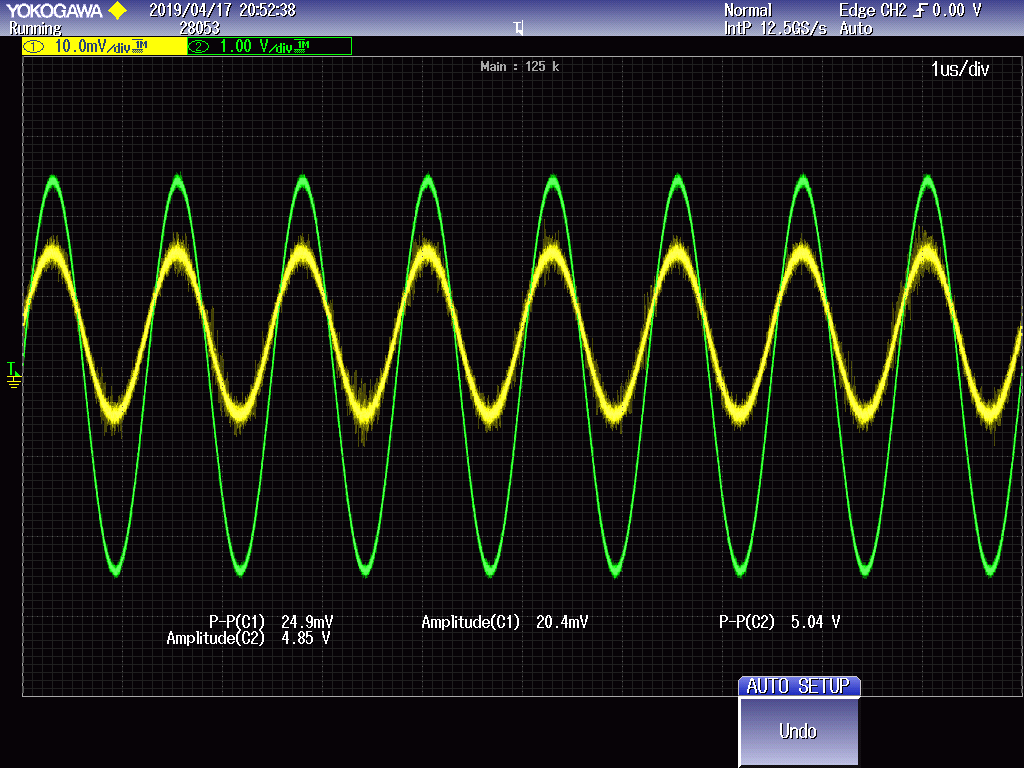
\includegraphics[width=\columnwidth]{images/lab8_012.png}
    \captionof{figure}{Phase shift at approximately 3kHz for the RC circuit}
    \label{fig:phaseshift40}
    \medskip
\endgroup

\section{Conclusions}
% Understanding and applications
\noindent As a result of this experiment, we learned how phases shift, not only based on the specification values of the reactive components, but also based on the frequency of the sinusoidal wave fed into the system. Furthermore, we learned that this frequency could be manipulated, to find the resonance frequency, in turn achieving a situation where there is no phase shift in current or voltage. The idea of resonance frequency can be used in circuits to act as a filter for certain ranges. For example, if the goal is to prevent a load from receiving certain frequencies, a tank circuit can act as a high impedance at that range of frequencies. \\

\noindent Ideally, an RC circuit can produce an output voltage with a phase shift of 90\degree. Combining two such circuits can be used to produce an output wave of 180\degree. However, practically speaking, as shown in this experiment, this is usually not the case. Hence, several stages can be used to achieve such an output. For example, three stages with a phase shift of 60\degree each, produces an RC oscillator, used in audio applications to convert DC signals to an AC signal. 

\printbibliography

\end{document}